\documentclass{article}
\usepackage{graphicx, amsmath, float, siunitx, hyperref, mathtools} % Required for inserting images
\usepackage[ngerman]{babel}
\usepackage{biblatex, csquotes}
\addbibresource{refs.bib}
\usepackage[
  locale=DE,
  separate-uncertainty=true,
  per-mode=symbol
]{siunitx}

\sisetup{output-decimal-marker = {,}}

\DeclareSIUnit\gauss{G}

\newcommand{\abb}{{\color{red}\textbf{{ABB.XYZ}}} }
\newcommand{\Oszi}{Oszilloskop }

\usepackage{caption}
\usepackage{subcaption}

\usepackage{csvsimple}
\usepackage{comment}
\usepackage{booktabs}

\title{Praktikum V - Kern- und Teilchenphysik\\Versuch 518 - Höhenstrahlung}

\author{Tom Chelius und Alican Özcagi}
\date{07. Mai 2025}


\begin{document}
\maketitle
\newpage
\tableofcontents

\newpage

\section{Einleitung}
Die Höhenstrahlung ist eine Form von ionisierender Strahlung, die in der Erdatmosphäre vorkommt. 
Sie besteht hauptsächlich aus hochenergetischen Teilchen, die aus dem Weltraum auf die Erde treffen. 
Diese Teilchen können Protonen, Elektronen und Atomkerne sein, die mit sehr hohen Geschwindigkeiten reisen. 
Die Höhenstrahlung entsteht durch verschiedene astrophysikalische Prozesse, wie z.B. Supernova-Explosionen oder 
die Wechselwirkung von kosmischer Strahlung mit der Erdatmosphäre.
In diesem Versuch werden wir die Höhenstrahlung auf seine Winkelverteilung untersuchen.
Außerdem werden wir die Lebensdauer der kosmischen Myonen bestimmen.

\section{Theorie}
Um diesen Versuch verstehen zu können, ist es wichtig, die Grundlagen der Höhenstrahlung und der Teilchhen zu kennen, sowie die 
Messinstrumente die wir verwenden werden. 

\subsection{Kosmische Strahlung}
Die kosmische Strahlung besteht aus hochenergetischen Teilchen, die aus verschiedenen Quellen stammen.
Sie kann hauptsächlich in 3 Kategorien unterteilt werden:
\begin{itemize}
    \item Teilchen die aus der Sonne stammen (Sonnenstrahlung) $\approx$ bis $\SI{10}{\giga\electronvolt}$
    \item Teilchen die aus dem interstellaren Raum stammen (Galaktische Strahlung) $\approx$ ab $\SI{1}{\giga\electronvolt}$ 
    \item Teilchen die aus dem intergalaktischen Raum stammen (Extragalaktische Strahlung)  $\approx$ bis $\SI{10}{\exa\electronvolt}$
\end{itemize}
Die Teilchen die auf die Erdatmosphäre treffen, sind hauptsächlich Elektronen, Photonen, Protonen und vollständig 
ioniersierte Kerne. Je nach Quelle sind die Energien der Teilchen unterschiedlich.
Die kosmische Strahlung wird in primäre und sekundäre Strahlung unterteilt.
Die primäre Strahlung sind die Teilchen die direkt aus dem Weltraum auf die Erde treffen.
Die sekundäre Strahlung sind die Teilchen die durch die Wechselwirkung der primären Strahlung mit der Erdatmosphäre entstehen.
Diese Entstehung der sekundären Strahlungen wird als Teilchenschauer bezeichnet, weil aus einem primären Teilchen viele sekundäre Teilchen entstehen. 
Sie wird aus den folgenden Prozessen gebildet:
\begin{itemize}
    \item \textbf{Kernreaktion:} Die Primäre Strahlung trifft auf die Atomkerne der Erdatmosphäre und erzeugt Sekundäre Teilchen.
    \item \textbf{Teilchenschauer:} Die Sekundären Teilchen erzeugen weitere Sekundäre Teilchen, die sich in alle Richtungen ausbreiten.
    \item \textbf{Ionisation:} Die Sekundären Teilchen ionisieren die Luftmoleküle und erzeugen weitere Elektronen.
\end{itemize}
Diese Teilchenschauer bestehten aus 3 Bereichen, wie in der Abbildung \ref{fig:Teilchenschauer} dargestellt.
\begin{figure}[H]
    \centering
    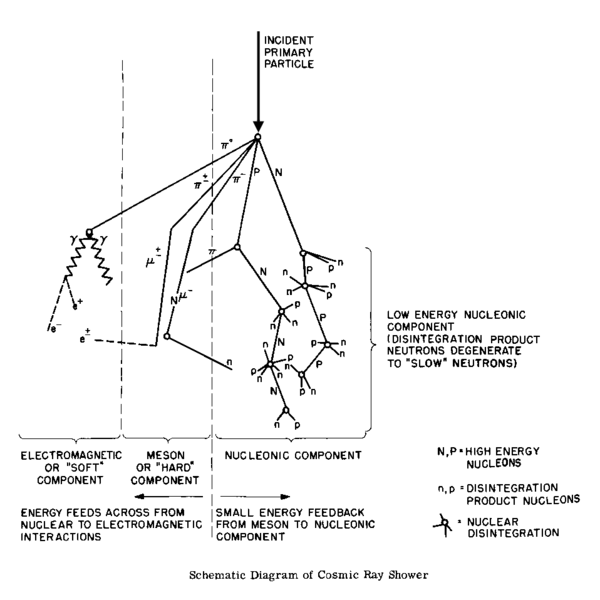
\includegraphics[width=0.5\textwidth]{figures/Teilchenschauer.png}
    \caption{Schematische Darstellung eines Teilchenschauers \cite{shower}}
    \label{fig:Teilchenschauer}
\end{figure}
\begin{itemize}
    \item Elektomagnetische-Komponente: Diese besteht aus Photonen und Elektronen und wird die \enquote{Softe} Komponente genannt.
    \item Mesonen-Komponente: Diese besteht aus Myonen und wird die "Harte" Komponente genannt.
    \item Nukleonen-Komponente: Diese besteht aus Protonen und Neutronen.
\end{itemize}
Die Teilchen die wir auf der Erdatmosphäre messen, sind hauptsächlich Myonen, da diese die Teilchen sind die mit am weitesten
in die Erdatmosphäre eindringen können und noch in hohen Quantitäten vorhanden sind.
In der Abbildung \ref{fig:Fluss} ist der vertikale Fluss zur atmosphärischen Eindringtiefe und zur Höhe der Erdoberfläche dargestellt.
\begin{figure}[H]
    \centering
    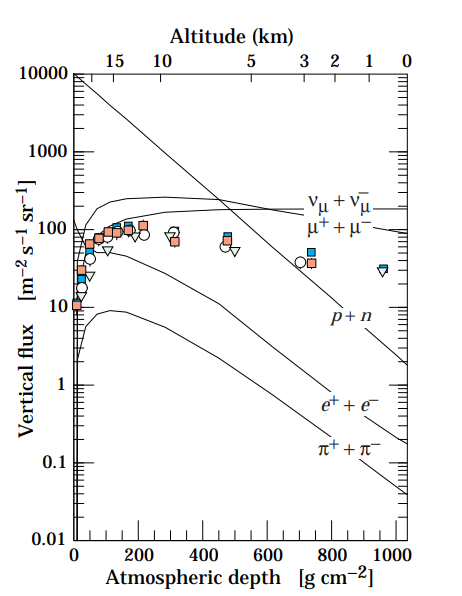
\includegraphics[width=0.5\textwidth]{figures/Fluss.png}
    \caption{Vertikaler Fluss zur atmosphärischen Eindringtiefe \cite{Naka}}
    \label{fig:Fluss}
\end{figure} 

\subsection{Standardmodell}
Das Standardmodell der Teilchenphysik ist eine Theorie, die die fundamentalen Teilchen und ihre Wechselwirkungen beschreibt.
Aus diesem können die Eigenschaften der Teilchen abgeleitet werden. Das Standardmodell ist in der Abbildung \ref{fig:Standardmodell} dargestellt.
\begin{figure}[H]
    \centering
    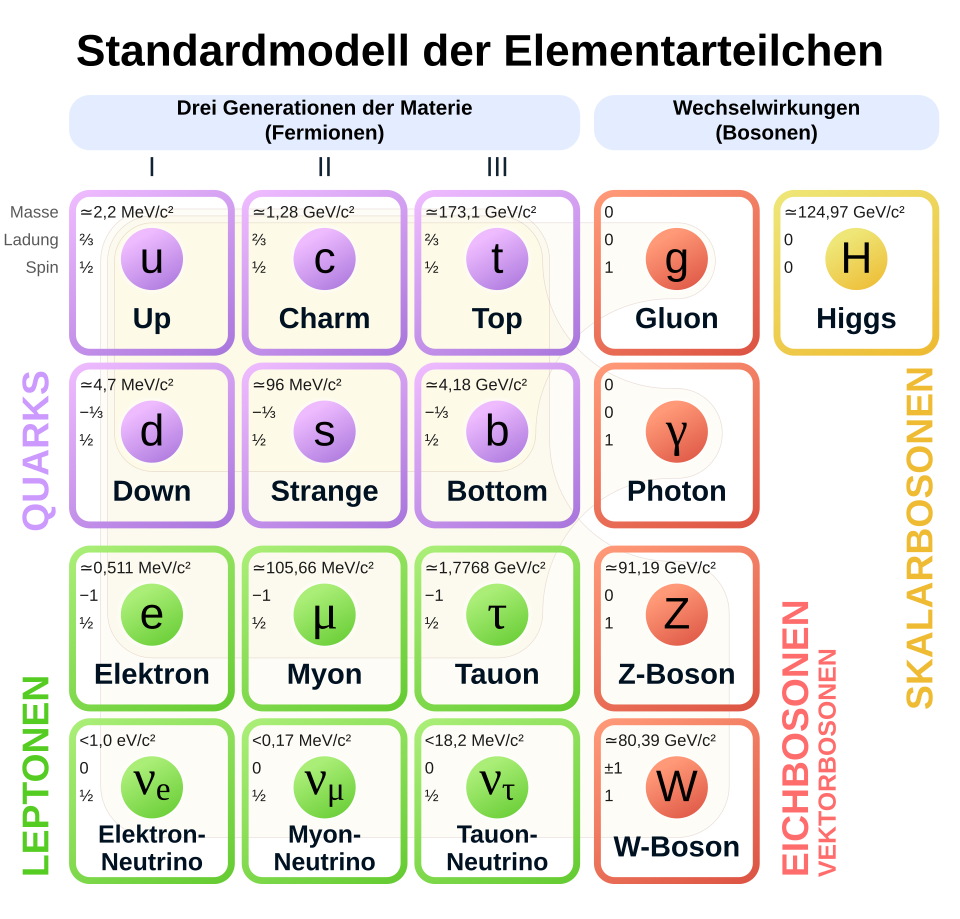
\includegraphics[width=0.5\textwidth]{figures/Standardmodell.png}
    \caption{Das Standardmodell der Teilchenphysik \cite{Standardmodell}}
    \label{fig:Standardmodell} 
\end{figure}
\textbf{\color{red}MEHR SCHREIBEN}

\subsection{Szintillator und Photomultiplier}
Szintillationsdetektoren basieren auf ausgesendeten Lichtteilchen (Photonen). Ionisierende Strahlung trifft auf das szintillierende Material und erzeugt durch Ionisation eine Kaskade an Elektron-Loch-Paaren. Dies geschieht durch Prozesse, wie im Abschnitt "Materie und Photonen Wechselwirkung" beschrieben. Die herausgelösten Elektronen überwinden somit die Bandlücke und landen im Leitungsband. Dort sind sie (sowie ihre hinerlassenen Löcher) als frei bewegliche Ladungen delokalisiert und können an anderer Stelle auf aktive Zentren stoßen. Diese aktiven Zentren kommen von der Dotierung mit einem anderen Material (hier Thallium) in unser Gitter. An diesen aktiven Zentren können sich die Elektron-Lochpaare über ein anderes Energieniveau lumineszierend abbauen, wobei Photonen im nahen bis sichtbaren Bereich ausgesendet werden. Wir verwenden in dem Versuch einen Natrium-Iod-Szintillationsdetektor den wir kurz NaI-Detektor nennen.

Der beschriebene Prozess ist auch nochmal in der Abbildung \ref{fig:SzintillatorBandlücke} dargestellt.


\begin{figure}
    \centering
    \includegraphics[width=1\linewidth]{Versuch 521/figures/Szintillator_Bändermodell.png}
    \caption{Darstellung des Bändermodell eines Szintillators \cite{Wer}}
    \label{fig:SzintillatorBandlücke}
\end{figure}

In dem Photomultiplier lösen die Photonen dann Elektronen aus der Photokathode. Eine Verstärkung wird über ein Dynodensystem realisiert. Hierbei gilt eine Dynode als Kathode, während die nächste als Anode wirkt und zwischen jedem Dynodenpaar wird das Signal verstärkt. Veranschaulicht wird der Effekt in der Abbildung \ref{fig:AufbauSzinti}. Der Photomultiplier ist an eine Hochspannungsquelle angeschlossen und die Dynoden haben über eine Reihe an Spannungsteilern zu immer höhere elektrische Potentiale.

\begin{figure}[H]
    \centering
    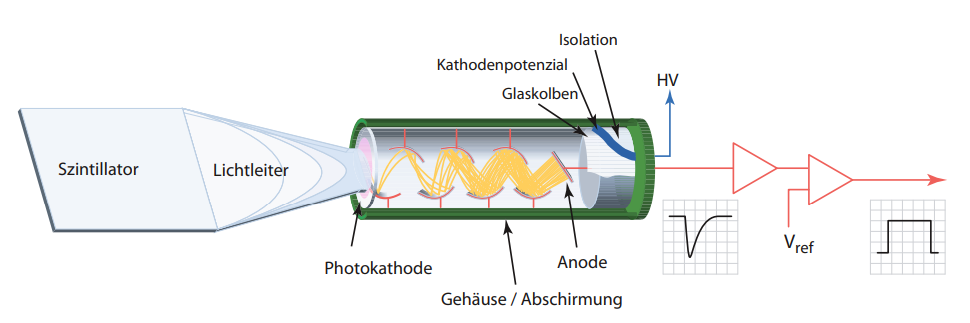
\includegraphics[width=1\linewidth]{Versuch 521/figures/SzintillatorAufbau.png}
    \caption{Aufbau eines Szintillator \cite{Wer}}
    \label{fig:AufbauSzinti}
\end{figure}

\subsection{Logische Schaltung: Diskriminator, Koinzidenz-Module und FPGA}
Um aus den gemessenen Analogen Signalen digitale Signale zu erzeugen, verwenden wir einen Diskriminator. 
Dieser trennt die Signale in zwei Bereiche: Ein Signal unterhalb der Schwelle wird als \enquote{0} und ein Signal oberhalb der Schwelle als "1" gewertet. 
Hiermit können wir Rauscheffekte vermeiden und zusätzlich gibt der Diskriminator uns die Möglichkeit, die Signaldauer einzustellen

Das Koinzidenz-Modul wirkt als ein logisches Und, es nimmt eine Menge an Signalen entgegen und gibt nur dann ein Signal aus, 
wenn alle Signale gleichzeitig anliegen. Das Koinzidenz-Modul wird verwendet damit einem durchfliegenden Teilchen ein Winkel zugeordnet werden kann, 
dazu wird geschaut, ob das Signal durch meherere Szintillatoren in einer Reihe gleichzeitig ausgelöst wird.

Ein FPGA (Field Programmable Gate Array) ist ein programmierbarer Logikbaustein und wird in diesem Versuch verwenden um Programme zu erstellen, die die Winkelverteilung
und die Lebensdauer der Myonen bestimmen können.
Die Programmierung wird in der LABView-Umgebung durchgeführt.
\subsection{Zufallskoinzidenz} 
Die Zufallskoinzidenz ist ein Effekt, der auftritt, wenn zwei oder mehr Ereignisse zufällig gleichzeitig auftreten. 
Dies ist relevant, weil wir bei der Bestimmung der Winkelverteilung und der Lebensdauer der Myonen wissen müssen, wie oft die Signale durch mehr als ein Teilchen
ausgelöst werden. Hierzu bestimmen wir die Zufallskoinzidenzrate um die Rate der echten Koinzidenzen zu bestimmen.
Diese kann auf 2 Arten bestimmt werden:
\begin{itemize}
    \item \textbf{zeitliche Zufallskoinzidenzrate:} Hierbei wird die Zeit der 3 Detektoren zeitlich so verschoben, dass ein einzelnes Teilchen keine Koinzidenz erzeugen kann.
        Es müssen also 3 Teilchen durch die 3 Detektoren fliegen um eine Koinzidenz zu erzeugen.
    \item \textbf{räumliche Zufallskoinzidenzrate:} Hierbei wird die räumliche Anordnung der Detektoren so gewählt, dass ein einzelnes Teilchen keine Koinzidenz erzeugen kann.
        Dabei müssen mindestens 2 Teilchen durch 2 Detektoren fliegen um eine Koinzidenz zu erzeugen.
\end{itemize}   

\section{Druchführung}

\section{Auswertung}

\newpage
\printbibliography[heading=bibintoc]

\end{document}